% !TeX root = ../thuthesis-example.tex

\chapter{信息整理与分析}

\section{数据来源}

\subsection{《中国药典》与中成药处方定量}

通过定量方法寻找有效的中药靶点,要求我们有足够的中药组成含量数据,而在临床实际中,往往并不是使用单一的中药,而是使用中医传统理论选取特定的中药组合,通过协同作用达到治疗目的。因此,我们需要的原始数据和模型最终的评估对象均为中药处方而非单一药材。这就需要足够数量的成分确定,且被临床实践确证有效的中药处方作为正例,而没有被实践选择的其他众多药材组合作为反例。《中国药典》作为一部有国家法律效力、规范包括中药在内国内药品生产和应用的权威性文件,其在中成药处方定量中的可用性高于古籍等其他资料;与此同时,它还以 HTML 网页的形式公开,非常方便进行数据的批量爬取,因此成为本研究处方-药材定量的主要依据。

\subsection{中药材定量数据库ccTCM}

严格来说,中药处方并不是各药材的简单混合,根据制剂类型的不同还可能涉及不同的提取、反应过程,但是在本研究中,我们无法建模这些复杂的处理过程,而认为经炮制后药材的成分含量结果可以基本反映最终生效的药物成分。这是后续的定量分析得以在处方-药材-化合物-基因的层级上进行的基本假设,否则就需要对每一种成药分别进行成分鉴定。此前,已经有多个项目对中药材的化合物组分进行了测定和整理,如 ccTCM, ITCM, BATMAN-TCM 等,而且相关论文均发表于近两年之内,具有较高的时效性。其中,ccTCM 提供较为完备的原始数据的下载,包括药材与其化合物组分、化合物与其可能影响表达的基因的关联表,可以进行离线分析,而不需要通过调用效率有限的 API,因此成为本研究中药材-化合物-基因定量的主要依据。

\subsection{蛋白互作网络STRING}

STRING, 即 Search Tool for the Retrieval of Interaction Gene/Proteins,是一个通用蛋白质互作网络数据库,包括多种生物体系的蛋白质互作关系,以及蛋白质与其他生物分子的关联。在本研究中,因为之前的两步数据整理已经将处方与具体基因联系起来,因此在基因层面我们可以不再依赖专门的中医药数据库,而可以使用更加通用的 STRING。STRING 可以针对一组输入的基因,返回它们之间的蛋白质互作网络,包括原始数据和可视化的形式,这对于我们在基因层面进行定量分析是非常有帮助的。

\section{《中国药典》处方收集整理}

《中国药典》全四部均可通过 \url{https://ydz.chp.org.cn} 获取,其组织形式非常有规律。对于我们需要的第一部中的中药数据,首先使用一个 URL 参数 \texttt{bookId=1},然后目录页即使用 \texttt{directoryId} 参数,第一部的目录范围为 1-16;内容页使用 \texttt{entryId} 参数,第一部的页码范围为 1-2282,其中 665-2282 即为我们需要的成方制剂和单味制剂,不再需要通过目录获取。因此,我们可以直接获取所有所需的静态页面进行分析,乃至本地部署使用。

对于药方这一层次结构且数据量较大的爬取对象,本步骤选用了 YAML 格式进行存储,从而实现了增量化存储,并有利于后续人工修改标注。存储层级为页码-处方名-处方药材及重量列表。页码信息有助于在归纳出热点处方之后回到《中国药典》进行反查。

在得到原始数据后,我们并无法直接使用得到的处方药材列表:一部分处方只给出了药材的名称而缺乏定量,另一部分给出的药材名称或者特定的制法无法在数据库中找到对应,这些数据无法使用,只能去除,或通过其他资料进行后续补充;中药的同物异名现象也影响到了药材的在数据库中的搜索,因此,我们需要借助中药学、植物学、矿物学等知识,在此基础上进行一定的人工整理。通过和在下一部分中介绍的 ccTCM 数据库进行对比,我们一共得到完整可用的处方 303 个,共涉及 156 味不同药材,从而限定了本研究的数据范围。

需要注意的是,如果能够通过结合其他文献或者进行实验的方式补充已知成分的药材列表,我们可以进一步扩大可用的处方范围,如下图为《中国药典》中处方在我们使用的ccTCM中缺失药材数据的分布情况:

\begin{figure}[H]
  \centering
  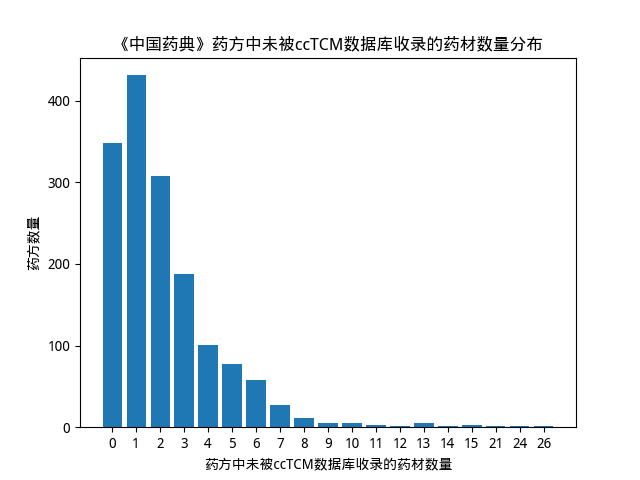
\includegraphics[width=0.8\textwidth]{figures/unlisted_medicinals_distribution}
  \caption{《中国药典》中处方在ccTCM中缺失药材数据的分布情况}
  \label{fig:missing_herbs}
\end{figure}

\section{ccTCM 数据库整理}

ccTCM 本身提供了使用中药、化合物或者基因靶标进行在线搜索的平台,但是这种访问方式不利于大规模的数据整理,因此我们选择了直接下载 ccTCM 的原始数据进行离线分析。这些数据以 TSV 格式存储在 \texttt{TCM\_information}, \texttt{Compound\_information}, \texttt{Target\_information} 这些基础信息文件和 \texttt{TCM\_compound-v1}, \texttt{Compound\_target-v1} 这两层关联文件之中,可以使用数据库合并的逻辑直接得到我们想要的信息,即药材中具体化合物的定量及特定化合物关联各基因的作用强度。其中,化合物定量往往可以给出一个具体的百分比范围,取其平均值进行后续计算即可,但是仅有 42\% 的化合物-基因关联存在以某种形式定量的作用强度,

而且存在量纲不一致、大量作用强度只使用占位值(如 $100000 \mathrm{nM}$ )的问题,几乎没有进行横向比较的可能,在本研究中只能暂时不考虑作用强度问题,或在某种程度上将其视为可学习的参数。我们实际得到的药材-基因定量关联权重是考虑所有与某种基因有关联的化合物,对它们在药材中的占比进行求和的结果,即:


$$
w_{\text{herb-gene}} = \sum_{\text{compound} \in \text{herb}} w_{\text{herb-compound}} \mathbf{1}_{\text{compound relates to gene}}
$$

\section{STRING查询与整理}

根据2024年5月31日的数据,STRING 数据库共收录 12535 种生物体的近 6000 万个蛋白质, 互作关系的规模大于 200 亿,是一个非常庞大的数据库,但是其提供了丰富的查询接口,并编写了详细的说明文档(\url{https://string-db.org/help/api/})。在这里,我们希望探究的是药材之前的相互作用,可分解为这样的子问题:遍历处方涉及的药材中的所有二元药材对,这两个药材关联基因的信息已经在前一步中获得,然后我们将这两个基因列表合并后调用STRING的 \texttt{network} API,就可以得到以原始 TSV 或 JSON 格式返回的基因互作分数网络,包括基因近邻分数、融合分数等多项细分关联度和STRING给出的一个综合分数,或者直接给出可视化图像。在我们已知